\section{Hardware architecture and configuration}
\paragraph{}
The TAKALEM Gloves, designed for \ac{slr}, consist of two main units: the sensing unit and the processing unit. This section focuses on the hardware architecture and configuration of these units, providing an overview of the components and their interconnections.
\paragraph{}
The sensing unit of the TAKALEM Gloves is responsible for capturing and collecting data related to hand movements and gestures. It comprises flex sensors and an MPU6050 sensor. The flex sensors are strategically positioned on the glove to measure the bend of individual fingers. They are connected to the microcontroller through designated pins, namely pins 13, 15, 25, 26, and 27. These flex sensors provide precise and real-time measurements of finger movements, allowing for accurate interpretation of \ac{sl} gestures.
\paragraph{}
In addition to the flex sensors, the TAKALEM Gloves also incorporate the MPU6050 sensor. The MPU6050 is an \ac{imu} that combines a three-axis accelerometer and a three-axis gyroscope. It measures the orientation and acceleration of the hand, providing valuable data for the \ac{slr} process. This sensor is connected to the microcontroller via the ASL (Accelerometer Serial Interface) and ASD (Accelerometer Serial Data) pins, enabling seamless data communication between the sensor and the processing unit.
\paragraph{}
The processing unit of the TAKALEM Gloves is powered by the ESP32 WROOM Module, a powerful microcontroller that integrates Wi-Fi and Bluetooth functionalities. This module acts as the brain of the gloves, processing the data collected from the flex sensors and the MPU6050 sensor. It is responsible for extracting and analyzing the sensor data, applying signal processing techniques, and calling the \ac{dl} model to predict the corresponding sign.
\paragraph{}
The ESP32 WROOM Module is equipped with sufficient computational power and memory to handle the complex algorithms and computations involved in real-time \ac{slr}. Its connectivity features allow for seamless integration with other devices, such as smartphones or smart home systems, enabling a wide range of applications.
\paragraph{}
To ensure optimal performance and reliable data transmission, the hardware components are carefully configured and calibrated. The flex sensors are positioned and secured on the glove to accurately measure finger bend without hindering natural hand movements. The MPU6050 sensor is properly calibrated to provide accurate orientation and acceleration data.
\paragraph{}
As a visual representation of the TAKALEM Gloves, \ref{fig:prototype} showcases the prototype of the gloves, highlighting the positioning of the flex sensors and the MPU6050 sensor. This prototype serves as a physical embodiment of the hardware architecture described in this section.
\begin{figure}[h]
	\centering
	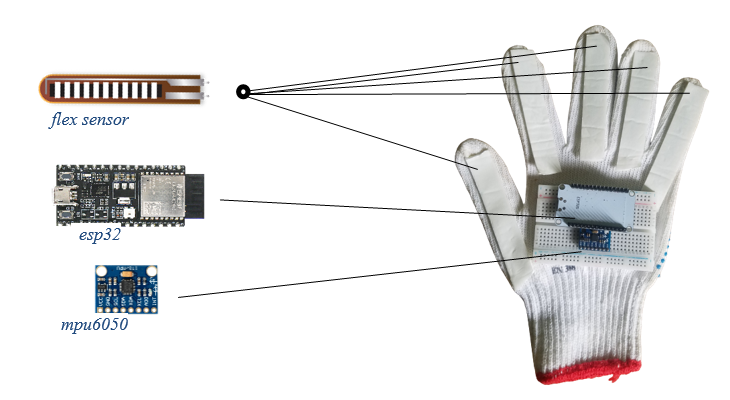
\includegraphics[width=0.7\linewidth]{images/prototype}
	\caption{TAKALEM Gloves components architecture}
	\label{fig:prototype}
\end{figure}
\subsection{ESP32 WROOM}
\paragraph{}
ESP32 is a highly versatile and powerful microcontroller \ac{soc} developed by Espressif Systems. It combines Wi-Fi and Bluetooth connectivity with a dual-core processor, making it ideal for various \ac{iot} applications.
\begin{figure}[h]
	\centering
	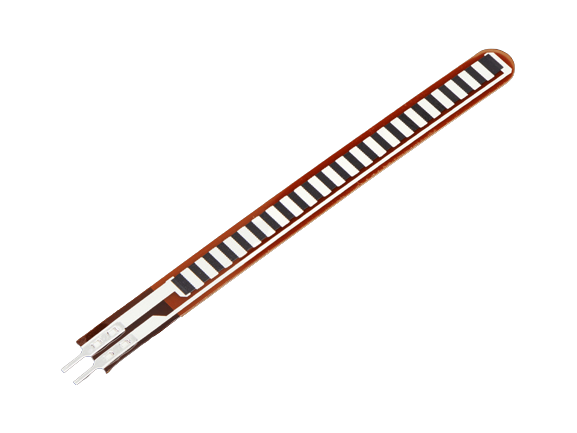
\includegraphics[width=0.5\linewidth]{images/flex-sensor}
	\caption{ESP32 WROOM}
	\label{fig:esp32}
\end{figure}
\subsection{Flex sensor}
\paragraph{}
Flex sensor is basically a variable resistor whose terminal resistance increases when the sensor is bent. So this sensor resistance increases depends on surface linearity. So it is usually used to sense the changes in linearity "\cite{flex}.
\begin{figure}[h]
	\centering
	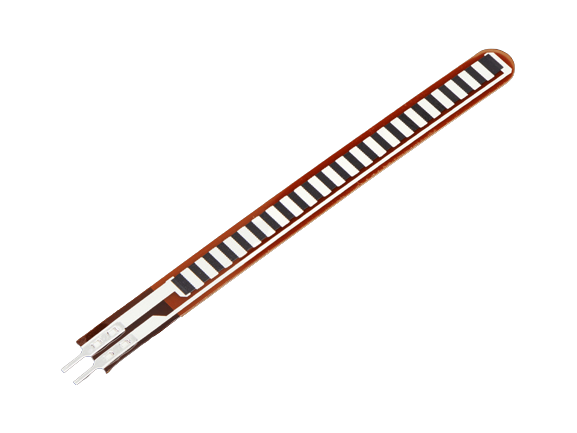
\includegraphics[width=0.5\linewidth]{images/flex-sensor}
	\caption{Flex sensor}
	\label{fig:flex-sensor}
\end{figure}
\paragraph{How flex sensor work}
As shown in figure \ref{fig:flex-cases}, when the surface of the flex sensor is completely linear it will be having its nominal resistance. When it is bent 45º angle the flex sensor resistance increases to twice as before. And when the bent is 90º the resistance could go as high as four times the nominal resistance. So the resistance across the terminals rises linearly with bent angle. So in a sense the flex sensor converts flex angle to resistance parameter "\cite{flex}.
\begin{figure}[h]
	\centering
	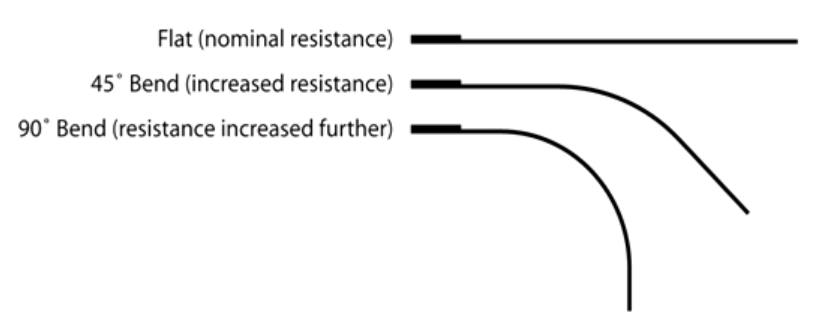
\includegraphics[width=0.5\linewidth]{images/flex-cases}
	\caption{Flex sensor cases "\cite{flex}}
	\label{fig:flex-cases}
\end{figure}
\paragraph{Flex sensor pinout}
The flex sensor is a two-way variable resistor with two pins, one for GND and the other for VCC. We wire one pin directly to the GND, the second pin is used to read the flex resistance via two wires, one is connected to the output pin in the esp32 and the other is connected to a constant resistance connected to the VCC.
\begin{figure}[h]
	\centering
	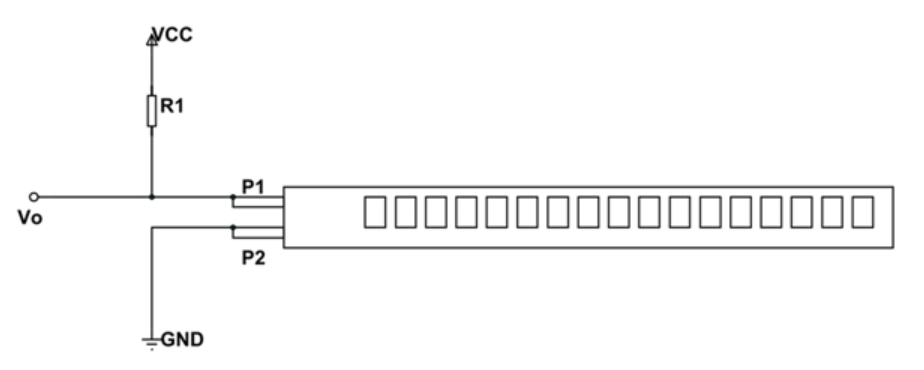
\includegraphics[width=0.5\linewidth]{images/flex-pinout}
	\caption{Flex sensor pin out}
	\label{fig:flex-pinout}
\end{figure}
\subsection{MPU6050}
\paragraph{}
The MPU6050 is a \ac{mems} which consists of a 3-axis Accelerometer and 3-axis Gyroscope inside it. This helps us to measure acceleration, velocity, orientation, displacement and many other motion related parameter of a system or object. This module also has a \ac{dmp} inside it which is powerful enough to perform complex calculation and thus free up the work for microcontrollers "\cite{mpu}.
\begin{figure}[h]
	\centering
	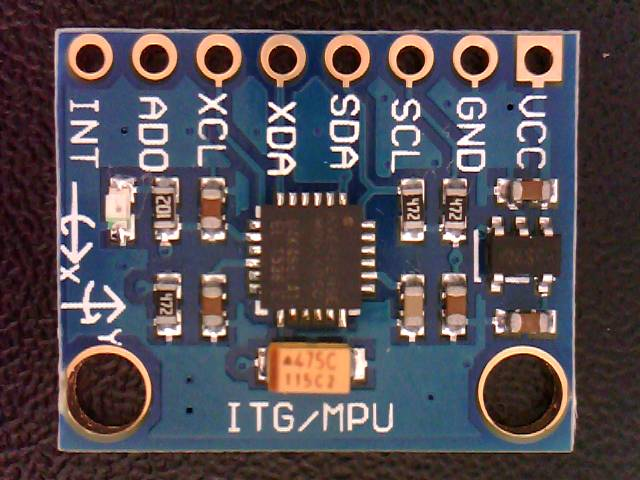
\includegraphics[width=0.5\linewidth]{images/mpu6050}
	\caption{MPU6050}
	\label{fig:mpu6050}
\end{figure}
\paragraph{MPU6050 pinout}
The MPU6050 sensor module and ESP32 have specific pinouts that need to be connected correctly. The MPU6050 typically has four important pins: VCC, GND, SDA, and SCL. The VCC pin is connected to a 3.3V or 5V output on the ESP32 to power the sensor. The GND pin of the MPU6050 is connected to a ground pin on the ESP32 to establish a common ground. The SDA pin of the MPU6050 is connected to the SDA pin on the ESP32 (pin D23), which handles the data line for I2C communication. Similarly, the SCL pin of the MPU6050 is connected to the SCL pin on the ESP32 (pin D21), which handles the clock line for I2C communication. It's important to make sure the correct pins are connected to establish proper communication between the MPU6050 and ESP32.
\begin{figure}[h]
	\centering
	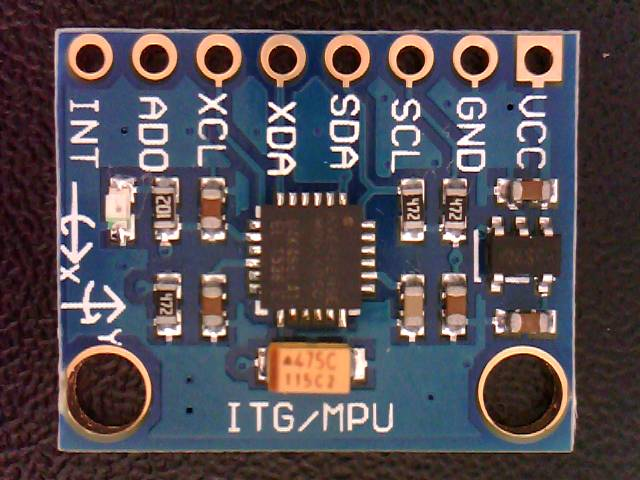
\includegraphics[width=0.5\linewidth]{images/mpu6050}
	\caption{MPU6050 pin out}
	\label{fig:mpu6050-pinout}
\end{figure}